\documentclass[11pt]{beamer}
\usepackage[utf8]{inputenc}
\usepackage[T1]{fontenc}
\usepackage{lmodern}
\usepackage[polish]{babel}
\usepackage{graphicx}
\usepackage{colortbl}
\usepackage{booktabs}
\usetheme{Warsaw}
%\usetheme{CambridgeUS}
%\usetheme{simple}
\definecolor{arsenic}{rgb}{0.0, 0.0, 0.142}
\usecolortheme[named=arsenic]{structure}
\newcommand*\oldmacro{}%
\let\oldmacro\insertshorttitle%
\renewcommand*\insertshorttitle{%
   \oldmacro\hfill%
   \insertframenumber\,/\,\inserttotalframenumber}


	\title{Kilka słów o prozodii semantycznej}
	\subtitle{Semantyka i poznanie}
	\author{Bartosz Maćkiewicz}

	\institute{Laboatorium Filozofii Eksperymentalnej KogniLab}
	\date{}
	%\subtitle{}
	%\logo{}
	%\subject{}
	%\setbeamercovered{transparent}
	%\setbeamertemplate{navigation symbols}{}
\begin{document}

\begin{frame}
\titlepage
\end{frame}

\begin{frame}
  \frametitle{Czteropoziomowy model rozszerzonej jednostki leksykalnej}
  \subtitle{Sinclair 1996, 1998}
  \textbf{OBSERWACJA}
  \begin{itemize}
	\item Użytkownicy języka posługują się bardzo dużą liczbą wzorców składania słów i tworzenia większych konstrukcji.
\end{itemize}
\end{frame}

\begin{frame}
  \frametitle{Czteropoziomowy model rozszerzonej jednostki leksykalnej}
  \subtitle{Sinclair 1996, 1998}
\textbf{ROZSZERZONA JEDNOSTKA LEKSYKALNA}
\begin{enumerate}
	\item Kolokacje
    \begin{itemize}
    \item często skonwencjonalizowane konstrukcje składające się ze słów, zwyczajowo występujących razem, np. ,,mocna herbata''
    \end{itemize}
	\item Koligacje
    \begin{itemize}
    \item systematyczne współwystępowanie danego słowa z jakąś konstrukcją składniową albo jakąś kategorią gramatyczną, np. ,,papier'' występuje często w konstrukcji ,,z papieru''
    \end{itemize}
	\item Preferencja semantyczna
    \begin{itemize}
    \item systematyczne współwystępowanie danego słowa z jakąś kategorią podobnych do siebie znaczeniowo słów, np. ,,jechać'' łączy się z klasą pojazdów, ,,the naked eye'' łączy się z czasownikami odnoszącymi się do percepcji wzrokowej
    \end{itemize}
	\item Prozodia semantyczna
    \begin{itemize}
    \item systematyczne współwystępowanie danego słowa z innymi jednostkami negatywnie lub pozytywnie nacechowanymi, np. ,,kompletny'' łączy się z negatywnie nacechowanymi rzeczownikami takimi jak ,,klapa'', ,,ruina'' lub ,,niewypał''
    \end{itemize}
\end{enumerate}
\end{frame}

\begin{frame}
  \frametitle{Prozodia semantyczna}
  \begin{itemize}
	\item Niektóre (zdawałoby się) neutralne słowa występują głównie w kontekstach wyraźnie nacechowanych negatywnie lub pozytywnie.
	\item Częste współwystępowanie wywołuje oczekiwanie, że kontekst, w którym znajduje się słowo, jest podobny do tego, w którym ono zazwyczaj występuje.
  \item Prozodia semantyczna niekoniecznie (w przeciwieństwie do klasycznie rozumianej ,,konotacji'') jest dostępna rodzimym użytkownikom języka w introspekcji
\end{itemize}
\end{frame}

\begin{frame}
  \frametitle{Przypadek ,,to cause''}
\textbf{Znacznie słownikowe}: \textit{make happen}

\vspace{1em}
\textbf{Przykłady z OED}
\begin{itemize}
	\item \textit{The difficult driving conditions caused several accidents.
		\item \textit{Most heart attacks are caused by blood clots.}}
	\item \textit{I hope the children haven't caused you too much trouble.}
\end{itemize}

\vspace{1em}
\textbf{Przykłady użycia z COCA}
\begin{figure}
	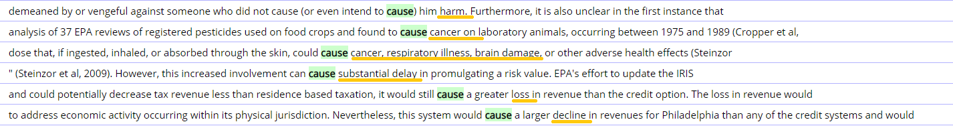
\includegraphics[scale=0.5]{uzycia_cause_coca}
\end{figure}
\vspace{1em}
\textbf{Negatywna prozodia ,,to cause''}: w 80\% wypadków ,,cause'' występuje w kontekstach negatywnych
\vspace{2em}
\end{frame}

\begin{frame}[t]
  \frametitle{Czy prozodia semantyczna ma realność psychologiczną?}
  \begin{itemize}
  \item Statystyczne obserwacje z korpusów tekstów niekoniecznie muszą być uważane za świadectwa na rzecz jakichś procesów poznawczych związanych z produkcją lub rozumieniem języka.
  \end{itemize}

  \vspace{1em}

  \textbf{Wnioski z wcześniejszych badań:}
  \begin{itemize}
  \item Produkcja wypowiedzi z pewnymi jednostkami semantycznymi jest wrażliwa na ich prozodię semantyczną (zadanie polegające na tworzeniu wypowiedzi ze słowem \textit{cause}, Nordquist 2004).
  \item Procesy rozpoznawania słów nie są wrażliwe na prozodię semantyczną (zadanie decyzji leksykalnych: Ellis, Frey, Jalkanen 2009).
  \item Prozodia semantyczna wpływa na przetwarzanie semantyczne (zadanie torowania afektywnego: Ellis, Frey, 2009).
  \end{itemize}
\end{frame}

\begin{frame}
  \frametitle{Czy prozodia semantyczna wpływa na sądy ocenne?}
  \begin{itemize}
  \item Działania są oceniane bardziej negatywnie, gdy ich opisy zawierają termin z negatywną prozodią niż wtedy, gdy jest to termin z prozodią pozytywną (bądź neutralną).
  \item Zjawisko to jest obecne nawet wtedy, gdy użytkownicy języka uważają, że terminy te oznaczają to samo i mają takie samo naładowanie ocenne.
  \item \textit{to cause} vs. \textit{to produce} (Hauser \& Schwarz 2016)
    \begin{itemize}
    \item Użytkownicy języka są bardziej skłonni do wywnioskowania z frazy ,,\textit{x} causes \textit{}y'', że \textit{y} jest czymś złym niż wtedy, gdy \textit{y} było \textit{produced}.
    \item Użytkownicy języka są bardziej skłonni do wywnioskowania z frazy ,,\textit{x} causes \textit{}y'', że \textit{x} miał intencję zrobienia \textit{y} niż wtedy, gdy \textit{y} było \textit{produced}.
    \item Użycie negatywnie naładowanego czasownika wpływa na przewidywania użytkowników języka co do prawdopodobieństwa wystąpienia skutku.
    \end{itemize}
  \end{itemize}
\end{frame}

\begin{frame}
  \frametitle{Metody określania prozodii semantycznej}
  W praktyce metodę określania prozodii semantycznej na podstawie korpusu można przedstawić w kilku krokach (procedura zaadaptowana z Kamasa 2015): 
  \begin{enumerate}
  \item Za pomocą odpowiedniego oprogramowania generuje się dla wybranego słowa listę kolakatów.
  \item Po wygenerowaniu listy ocenia się znajdujące się na niej kolokaty ze względu na nacechowanie. Językoznawcy spierają się co do tego, czy prozodia semantyczna polega tylko na negatywnym, pozytywnym lub neutralnym nacechowaniu (por. Bańko 2008), ale te trzy kategorie są przyjmowane najczęściej.
  \item Jeżeli nacechowanie któregoś z kolokatów jest niejasne, należy sprawdzić szerszy kontekst jego użycia wraz z interesującym nas słowem i na tej podstawie dokonać oceny.
  \item Prozodią semantyczną badanego przez nas słowa jest nacechowanie, które dominuje wśród kolokatów.
  \end{enumerate}
\end{frame}

\begin{frame}
  \frametitle{Dodatkowe kryteria}
  \begin{block}{Konstruowanie listy kolokatów}
    Niektórzy badacze (Mautner 2007, Walker 2011) zalecają, aby z takiej listy wyeliminować kolokaty o niskim współczynniku kolokacji oraz takie, które mają niską częstotliwość występowania.

    Można ograniczyć się również tylko do określonych cześci mowy albo uwzględnić słowa nie tylko występujące w bezpośrednim sąsiedztwie, ale również  te znajdujące się w odległości kilku słów od badanej przez nas jednostki.
  \end{block}
\end{frame}

\begin{frame}
  \Huge
  \resizebox{\linewidth}{!}{Dziękuję za uwagę!}

\end{frame}
\end{document}